\chapter{Coordinate Transformation}\label{ch:appendix1}

For a mobile robot, a point $\boldsymbol{P}$ in space has
coordinates $[\begin{matrix}x & y & z\end{matrix}]$ in the world frame, and
$[\begin{matrix}x' & y' & z' \end{matrix}]$ in the mobile frame, as
illustrated in Figure \ref{fig:appx1-1}

\begin{figure}[h]
\centering
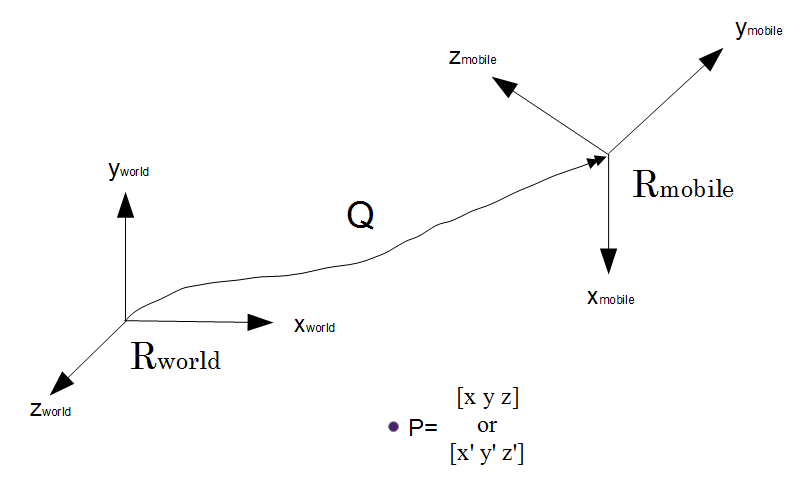
\includegraphics[width=12cm, keepaspectratio=true]{./Figures/coordinate_transformation/coordinate_transformation.png}
\caption{A point in the world frame and the mobile frame}
\label{fig:appx1-1}
\end{figure}

The coordinates for the same point $\boldsymbol{P}$ in the world frame
and the mobile frame are related by
\begin{equation}
\begin{bmatrix}
x \\ y \\ z \\ 1 \\
\end{bmatrix}_{World}=\boldsymbol{Q}\cdot\begin{bmatrix}
x' \\ y' \\ z' \\ 1  \\
\end{bmatrix}_{mobile}
\end{equation}

\noindent where $\boldsymbol{Q}$ is the transformation matrix composed
of rotation and translation that evolve the world frame to the mobile frame. The
calculation of $\boldsymbol{Q}$ must follow the TRPY (translate-roll-pitch-yaw)
convention, hence $\boldsymbol{Q}$ is given by

\begin{equation}
\boldsymbol{Q}= \boldsymbol{Q_TQ_{R_z}Q_{R_y}Q_{R_x}}
\end{equation}

$\boldsymbol{Q_T}$, $\boldsymbol{Q_{R_x}}$, $\boldsymbol{Q_{R_y}}$,
$\boldsymbol{Q_{R_z}}$ are the translation and rotation matrices for axes
$X$, $Y$ and $Z$. They are give in Equation (\ref{eq:translate}) to
(\ref{eq:rotz}).

\begin{equation}
\label{eq:translate}
\boldsymbol{Q_T} = \begin{bmatrix}
1 & 0 & 0 & x_T \\
0 & 1 & 0 & y_T \\
0 & 0 & 1 & z_T \\
0 & 0 & 0 & 1 \end{bmatrix}
\end{equation}

\begin{equation}
\label{eq:rotx}
\boldsymbol{Q_{R_x}}= \begin{bmatrix}
1 & 0 & 0 & 0 & \\
0 & \cos (r_{x}) & -\sin (r_{x}) & 0 & \\
0 & \sin (r_{x}) & \cos (r_{x}) & 0 & \\
0 & 0 & 0 & 1 & \\
\end{bmatrix}
\end{equation}


\begin{equation}
\label{eq:roty}
\boldsymbol{Q_{R_y}}= \begin{bmatrix}
\cos (r_{y}) & 0 & \sin (r_{y}) & 0 & \\
0 & 1 & 0 & 0 & \\
-sin(r_{y}) & 0 & \cos (r_{y}) & 0 & \\
0 & 0 & 0 & 1 & 
\end{bmatrix}
\end{equation}


\begin{equation}
\label{eq:rotz}
\boldsymbol{Q_{R_z}}=\begin{bmatrix}
\cos (r_{z}) & -\sin (r_{z}) & 0 & 0 & \\
\sin (r_{z}) & \cos (r_{z}) & 0 & 0 & \\
0 & 0 & 1 & 0 & \\
0 & 0 & 0 & 1 & \\
\end{bmatrix}
\end{equation}

The forward transformation calculates point $\boldsymbol{P}$'s
coordinates in the world frame given its location in the mobile frame.
To calculate point $\boldsymbol{P}$'s coordinates in the mobile frame
from its location in the world frame, inverse transformation can
be used. The inverse transformation matrix is given in Equation
(\ref{eq:Qinv}) - (\ref{eq:rotz_inv})

\begin{equation}
\label{eq:Qinv}
\boldsymbol{Q}^{-1}=\boldsymbol{Q_{R_x}}^{-1}\boldsymbol{Q_{R_y}}^{-1}
\boldsymbol{Q_{R_z}}^{-1} \boldsymbol{Q_T}^{-1}
\end{equation}

\begin{equation}
\label{eq:translate_inv}
\boldsymbol{Q_{T}}^{-1}=\begin{bmatrix}
1 & 0 & 0 & -x_T \\
0 & 1 & 0 & -y_T \\
0 & 0 & 1 & -z_T \\
0 & 0 & 0 & 1\end{bmatrix}
\end{equation}

\begin{equation}
\label{eq:rotx_inv}
\boldsymbol{Q_{R_x}}^{-1}=\boldsymbol{Q_{R_x}}^{T}
\end{equation}

\begin{equation}
\label{eq:roty_inv}
\boldsymbol{Q_{R_y}}^{-1}=\boldsymbol{Q_{R_y}}^{T}
\end{equation}

\begin{equation}
\label{eq:rotz_inv}
\boldsymbol{Q_{R_z}}^{-1}=\boldsymbol{Q_{R_z}}^{T}
\end{equation}




%%% Local Variables:
%%% mode: latex
%%% TeX-master: "thesis"
%%% End:
